
%NOTE: to be used with \usepackage{subfiles} in the main file.
%Subfiles go in folders which live with the main file.
%Bibliography and preamble go in the main file.

%%%%%%%%%%%%%%%%%%%%%%%% PREAMBLE %%%%%%%%%%%%%%%%%%%%%%%%
\providecommand{\main}{..}

\documentclass[main]{subfiles} %Each instance of `../' elevates one folder to find the main file

\begin{document}

%%%%%%%%%%%%%%%%%%%%%%% DOCUMENT %%%%%%%%%%%%%%%%%%%%%%%

% \tableofcontents % Can be useful to load a TOC while writing

\doublespacing

\schapter{Results}
\label{sect:results}
\vspace{20pt}

An initial assessment of the discriminant capabilities of the substructure variables studied in this work can be done by looking at the difference in their distributions for signal and background events. The distributions for multiple fat jet variables in the training sample events for both the top signal and the QCD background are shown in figure \ref{fig:top_distributions}.\\

As can be seen from (a) - (d) tauN is BAD \dots


\dots It should be noted that these were produced with the parton cut of 350gev and a R of 1.0


\begin{figure}[h]
     \centering
     \begin{subfigure}[h]{0.49\textwidth}
         \centering
         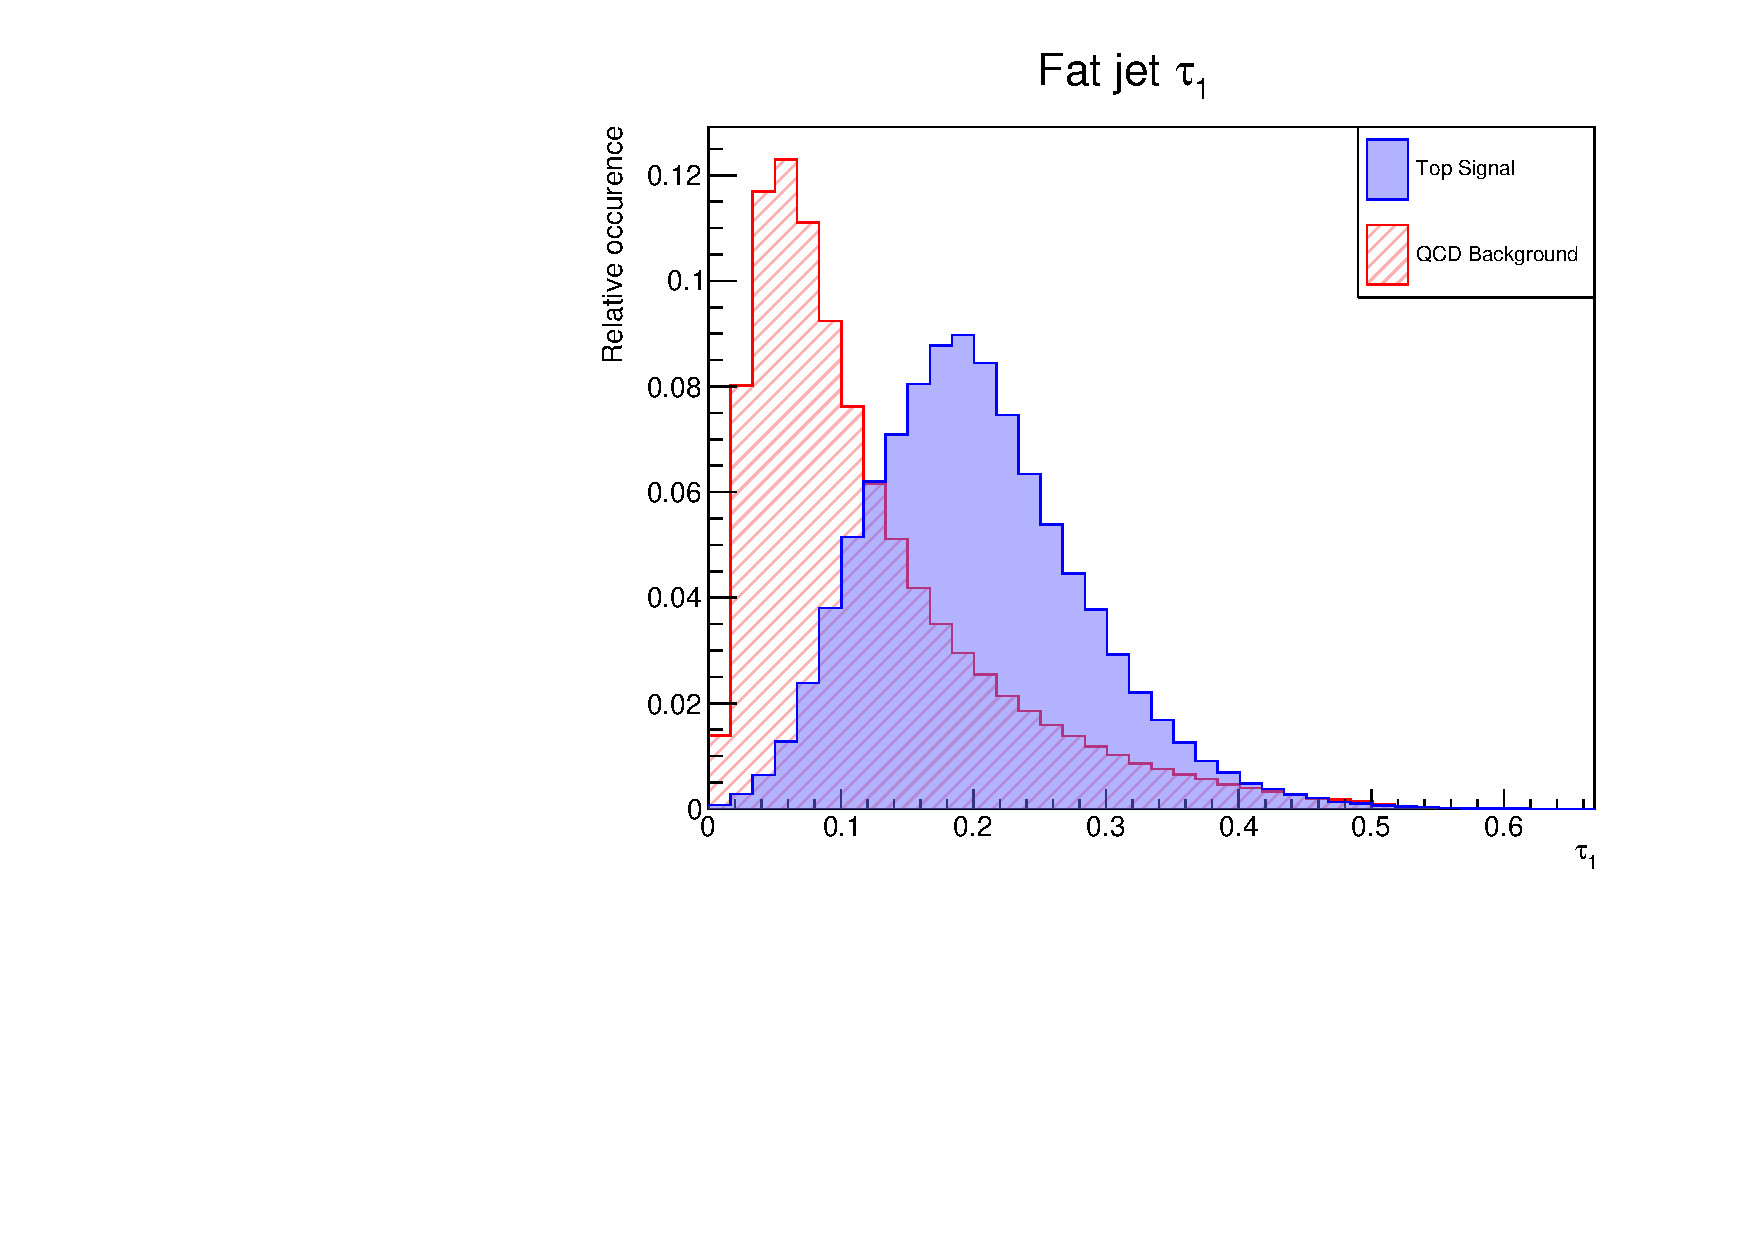
\includegraphics[width=0.8\textwidth]{../Figures/Results/top_distributions/top_tau1_distribution.pdf}
          \caption{}
         \label{fig:top_distribution_tau1}
     \end{subfigure}
     \begin{subfigure}[h]{0.49\textwidth}
         \centering
         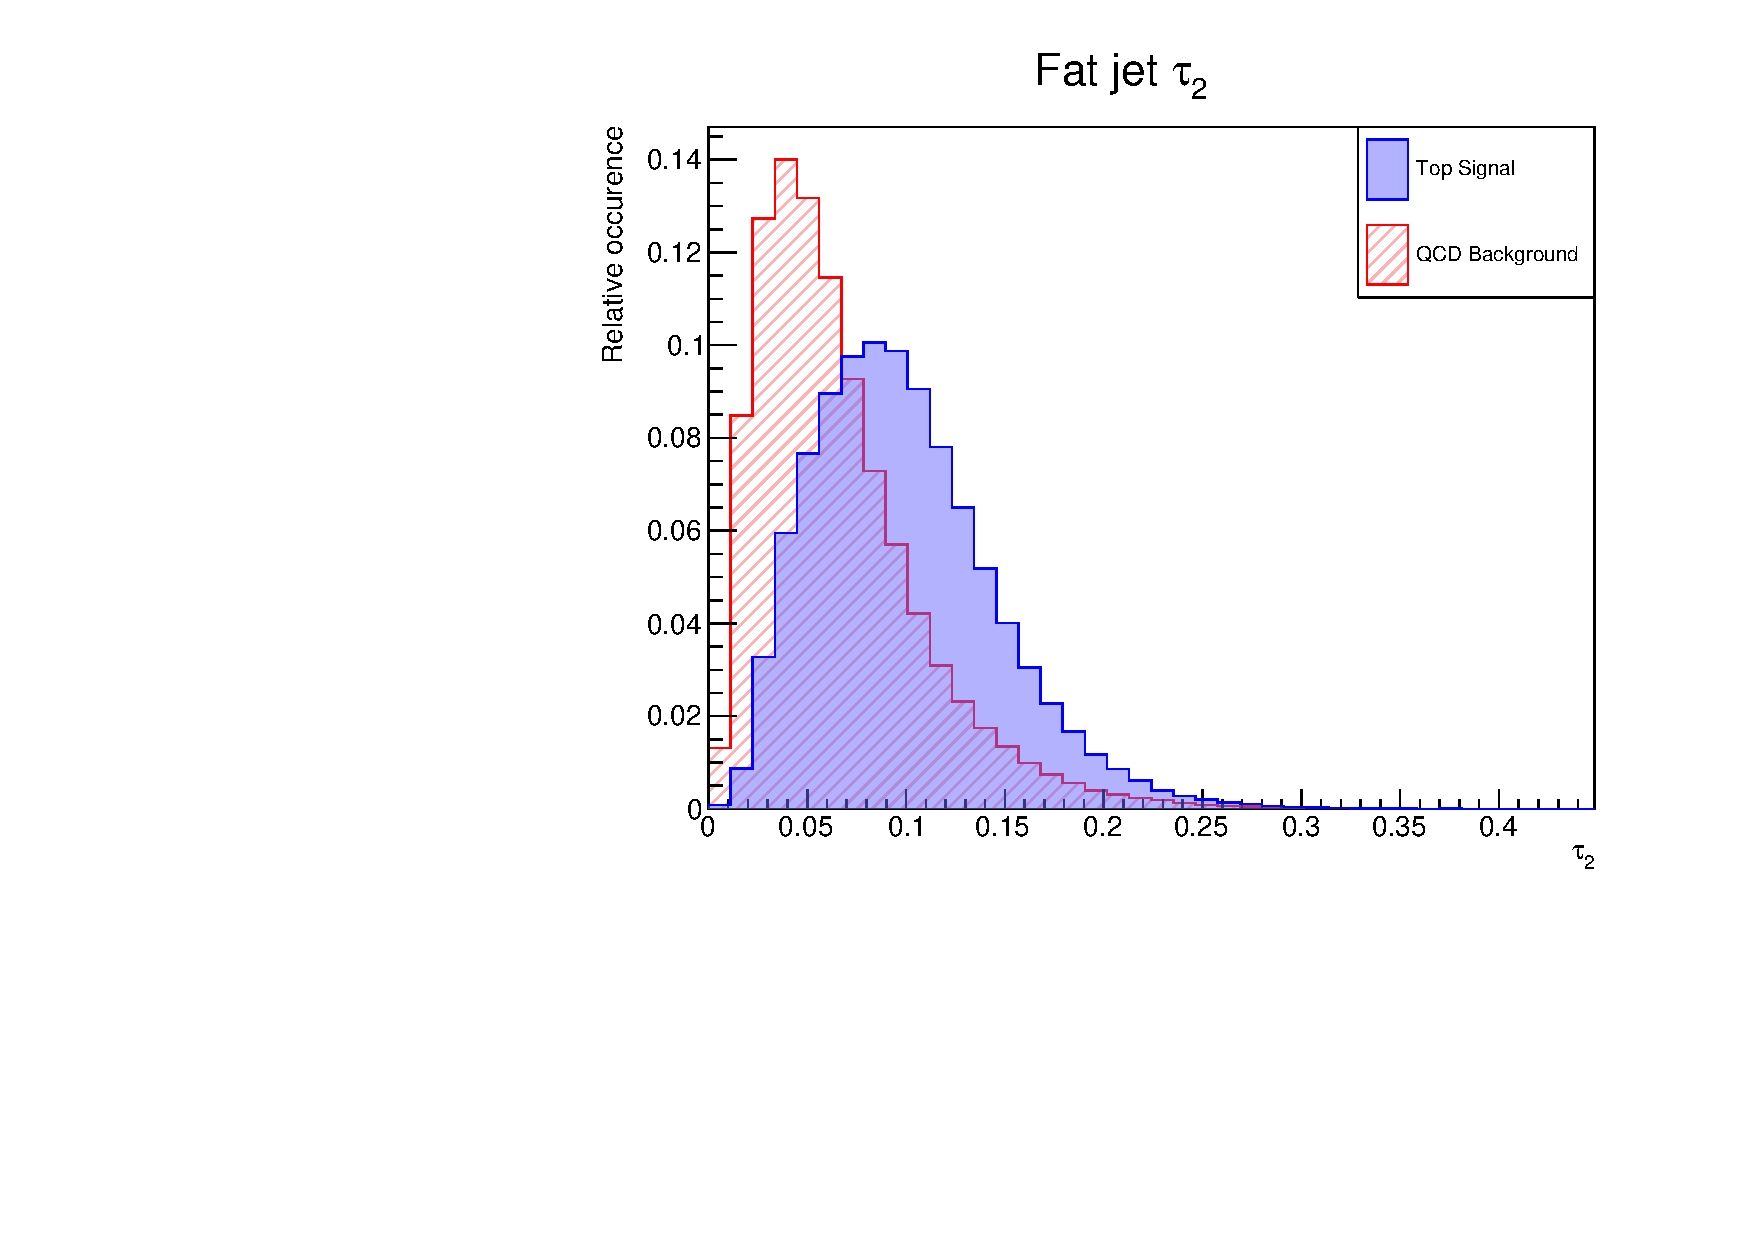
\includegraphics[width=0.8\textwidth]{../Figures/Results/top_distributions/top_tau2_distribution.pdf}
          \caption{}
         \label{fig:top_distribution_tau2}
     \end{subfigure}
     \par\bigskip
     \begin{subfigure}[h]{0.49\textwidth}
         \centering
         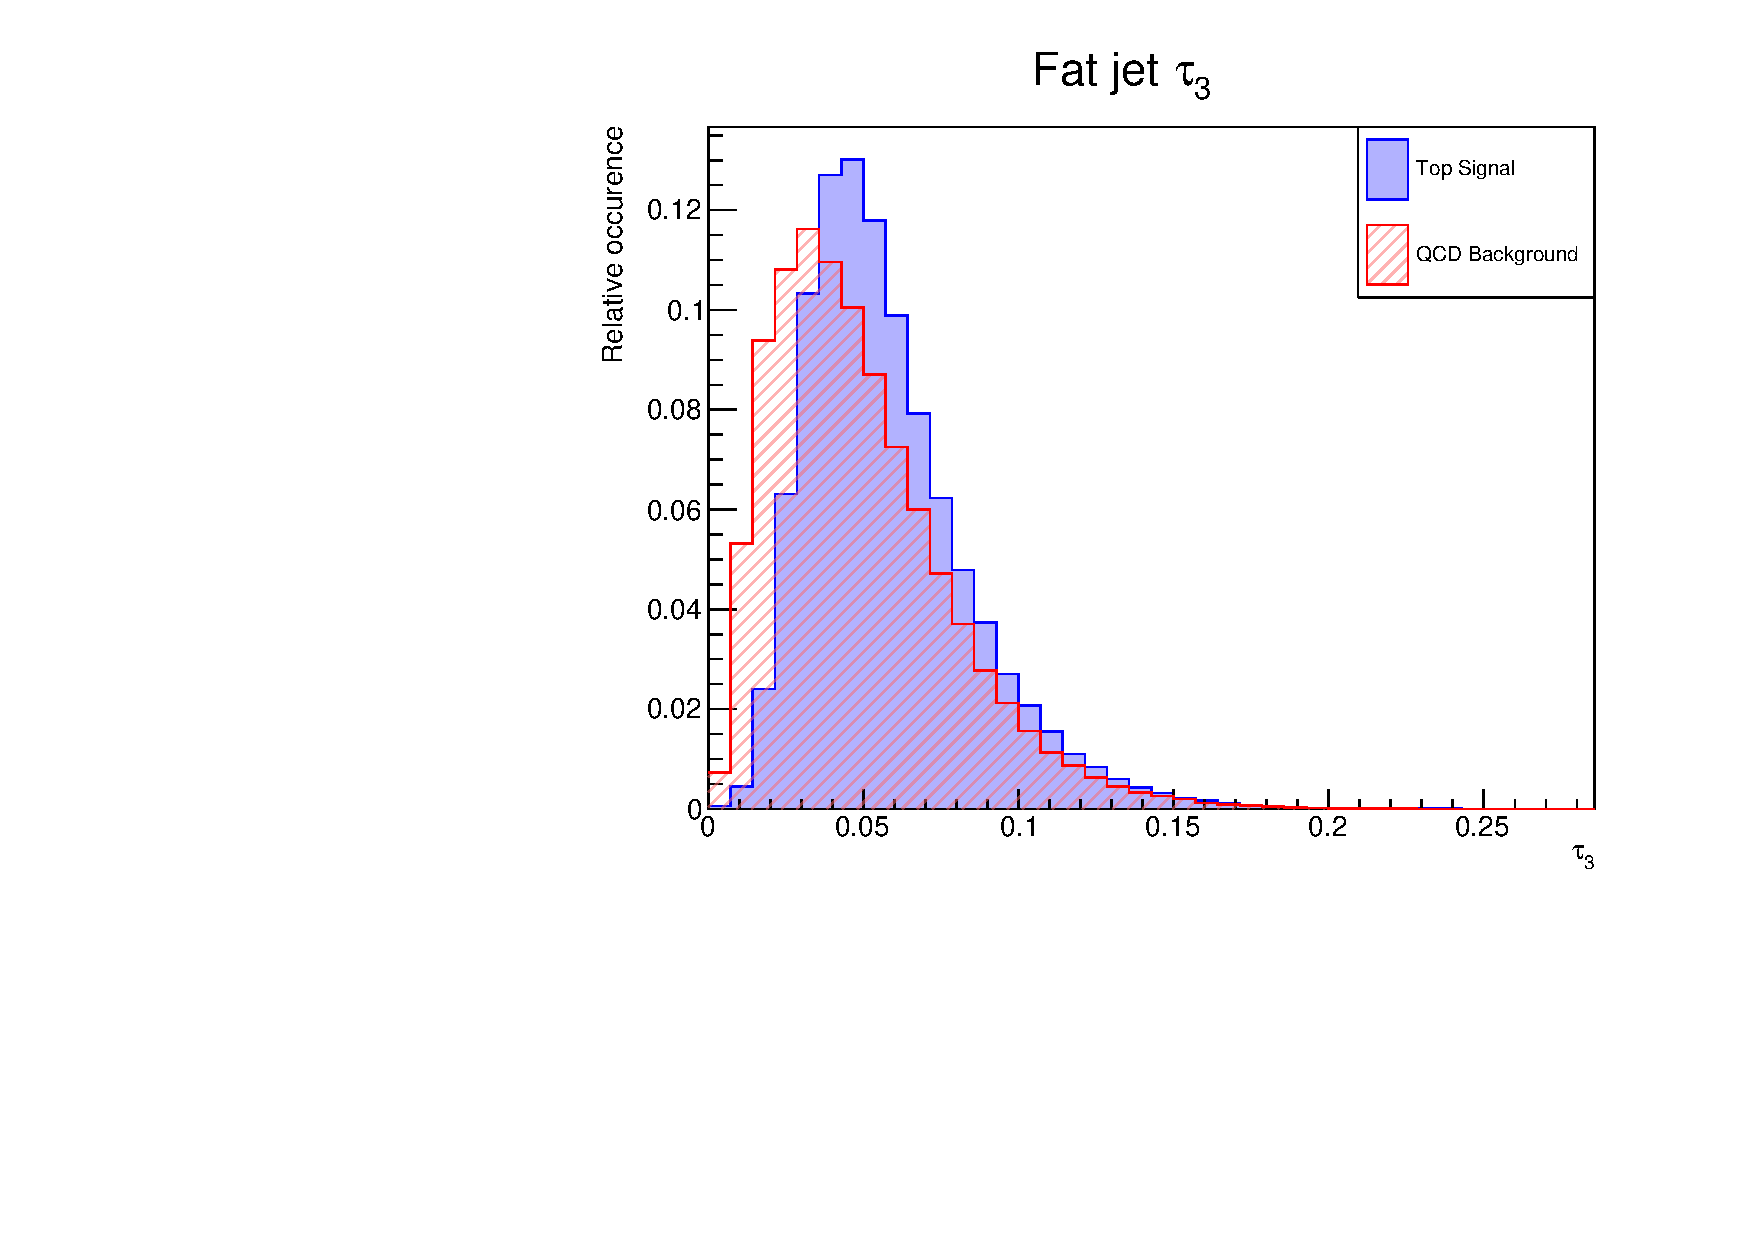
\includegraphics[width=0.8\textwidth]{../Figures/Results/top_distributions/top_tau3_distribution.pdf}
          \caption{}
         \label{fig:top_distribution_tau3}
     \end{subfigure}
     \begin{subfigure}[h]{0.49\textwidth}
         \centering
         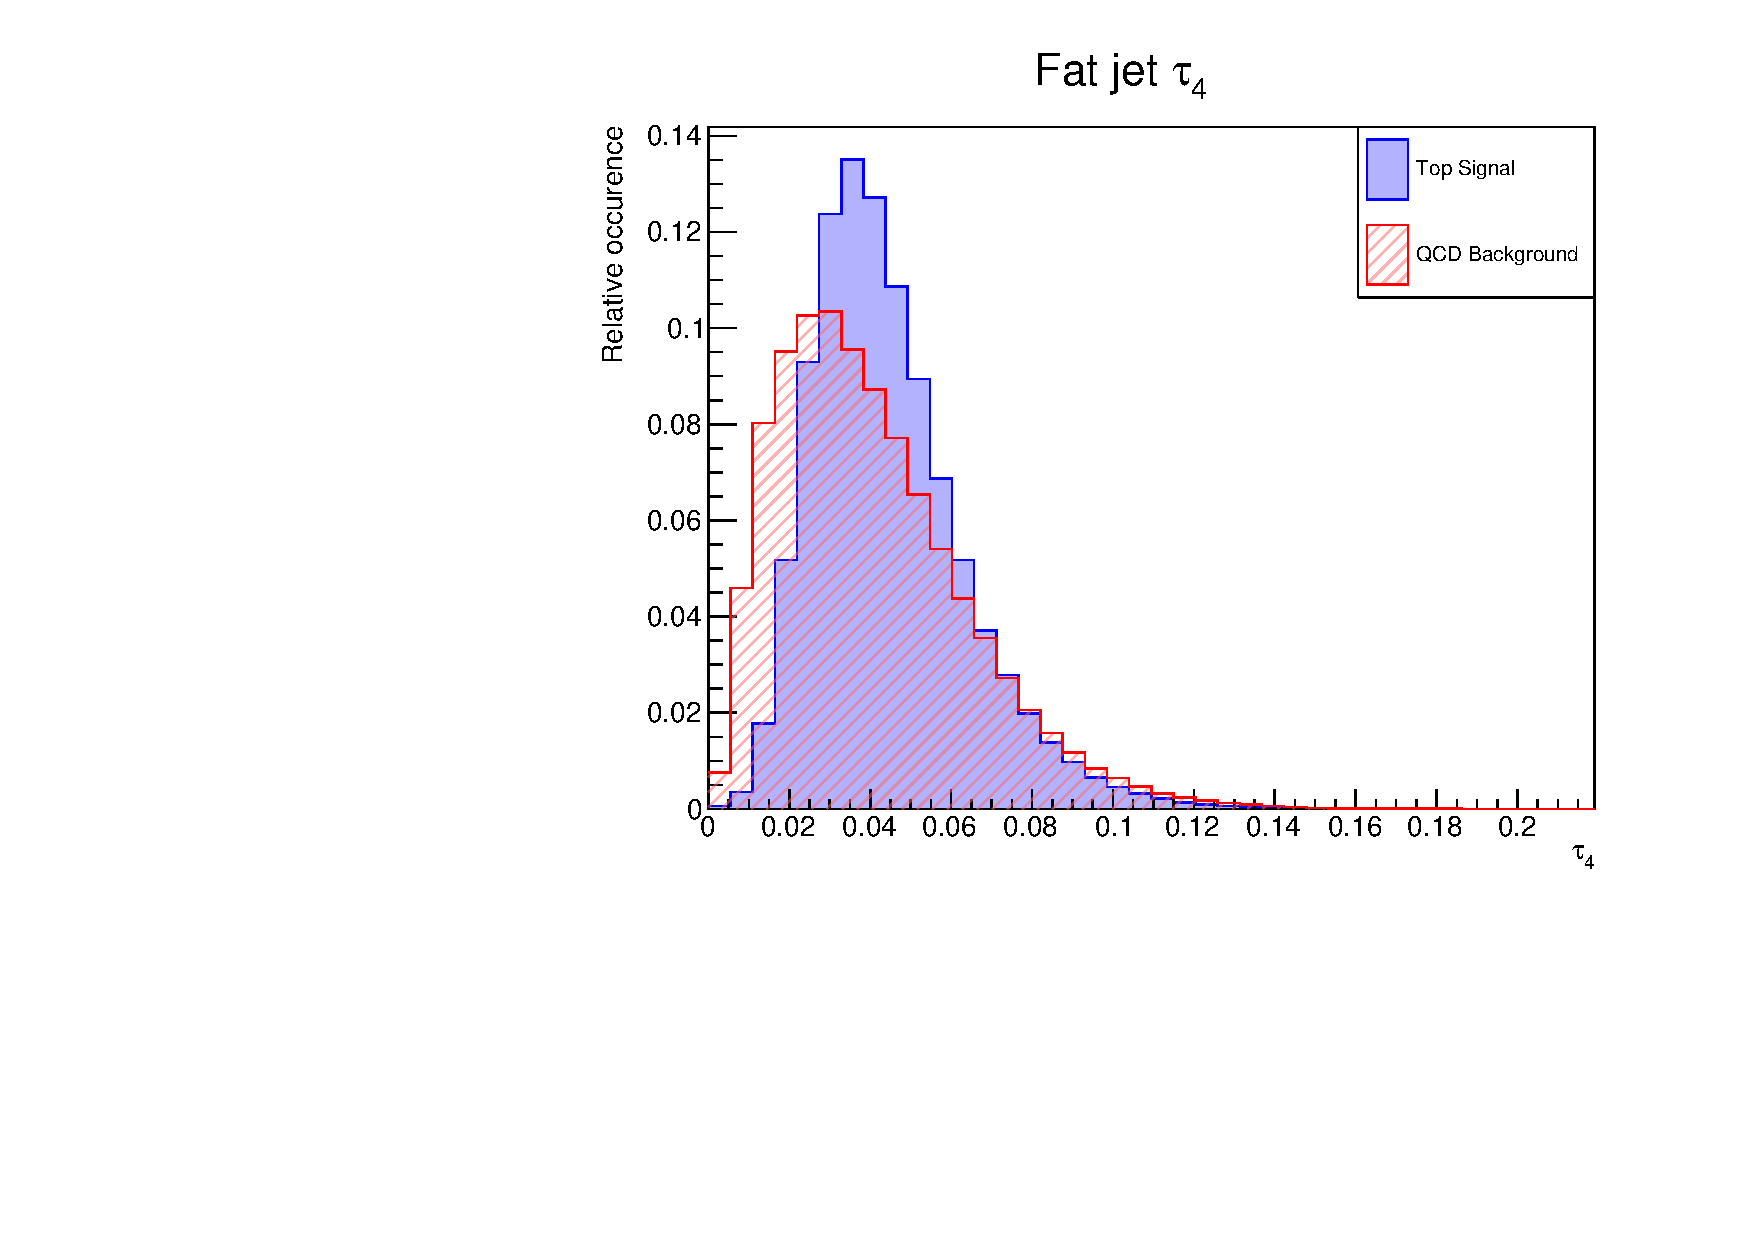
\includegraphics[width=0.8\textwidth]{../Figures/Results/top_distributions/top_tau4_distribution.pdf}
          \caption{}
         \label{fig:top_distribution_tau4}
     \end{subfigure}
     \par\bigskip
     \begin{subfigure}[h]{0.49\textwidth}
         \centering
         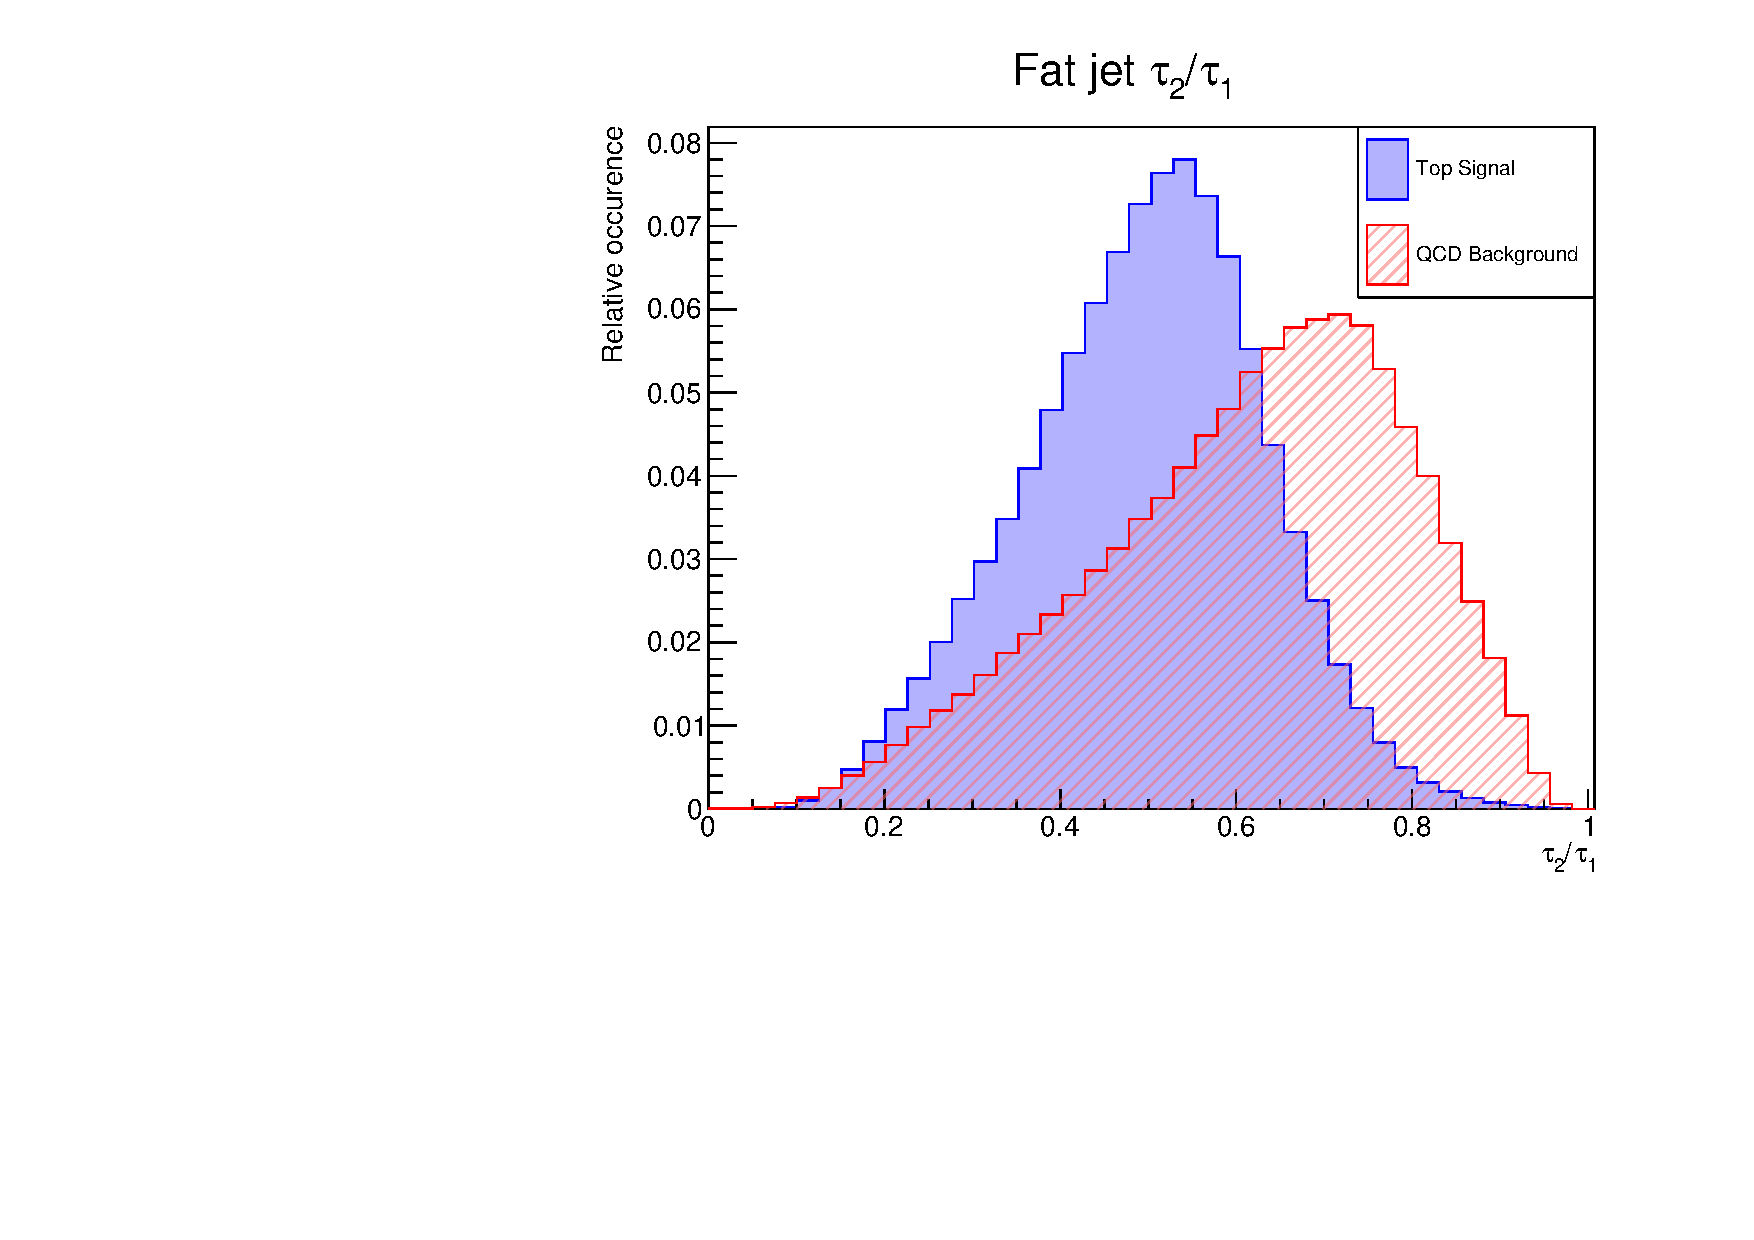
\includegraphics[width=0.8\textwidth]{../Figures/Results/top_distributions/top_tau21_distribution.pdf}
          \caption{}
         \label{fig:top_distribution_tau21}
     \end{subfigure}
     \begin{subfigure}[h]{0.49\textwidth}
         \centering
         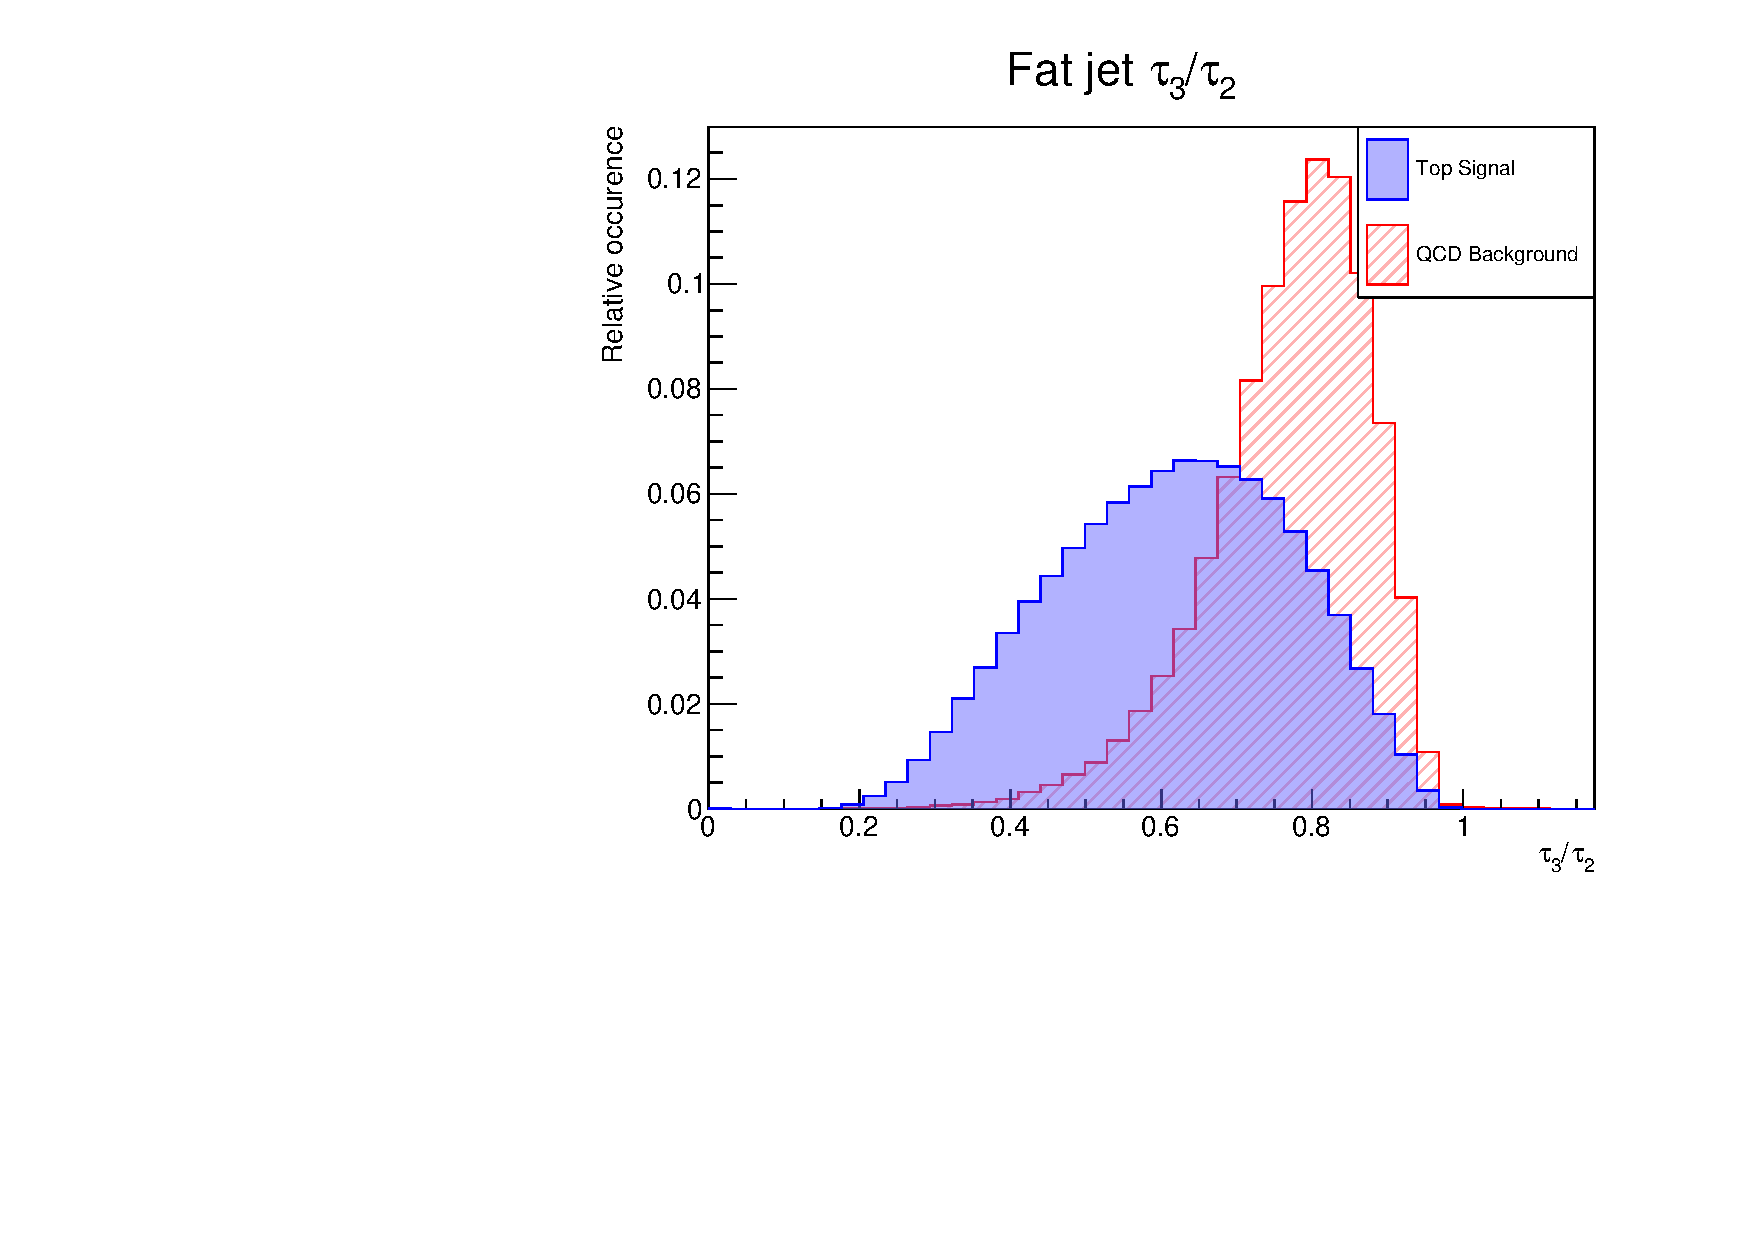
\includegraphics[width=0.8\textwidth]{../Figures/Results/top_distributions/top_tau32_distribution.pdf}
          \caption{}
         \label{fig:top_distribution_tau32}
     \end{subfigure}
     \par\bigskip 
     \begin{subfigure}[h]{0.49\textwidth}
         \centering
         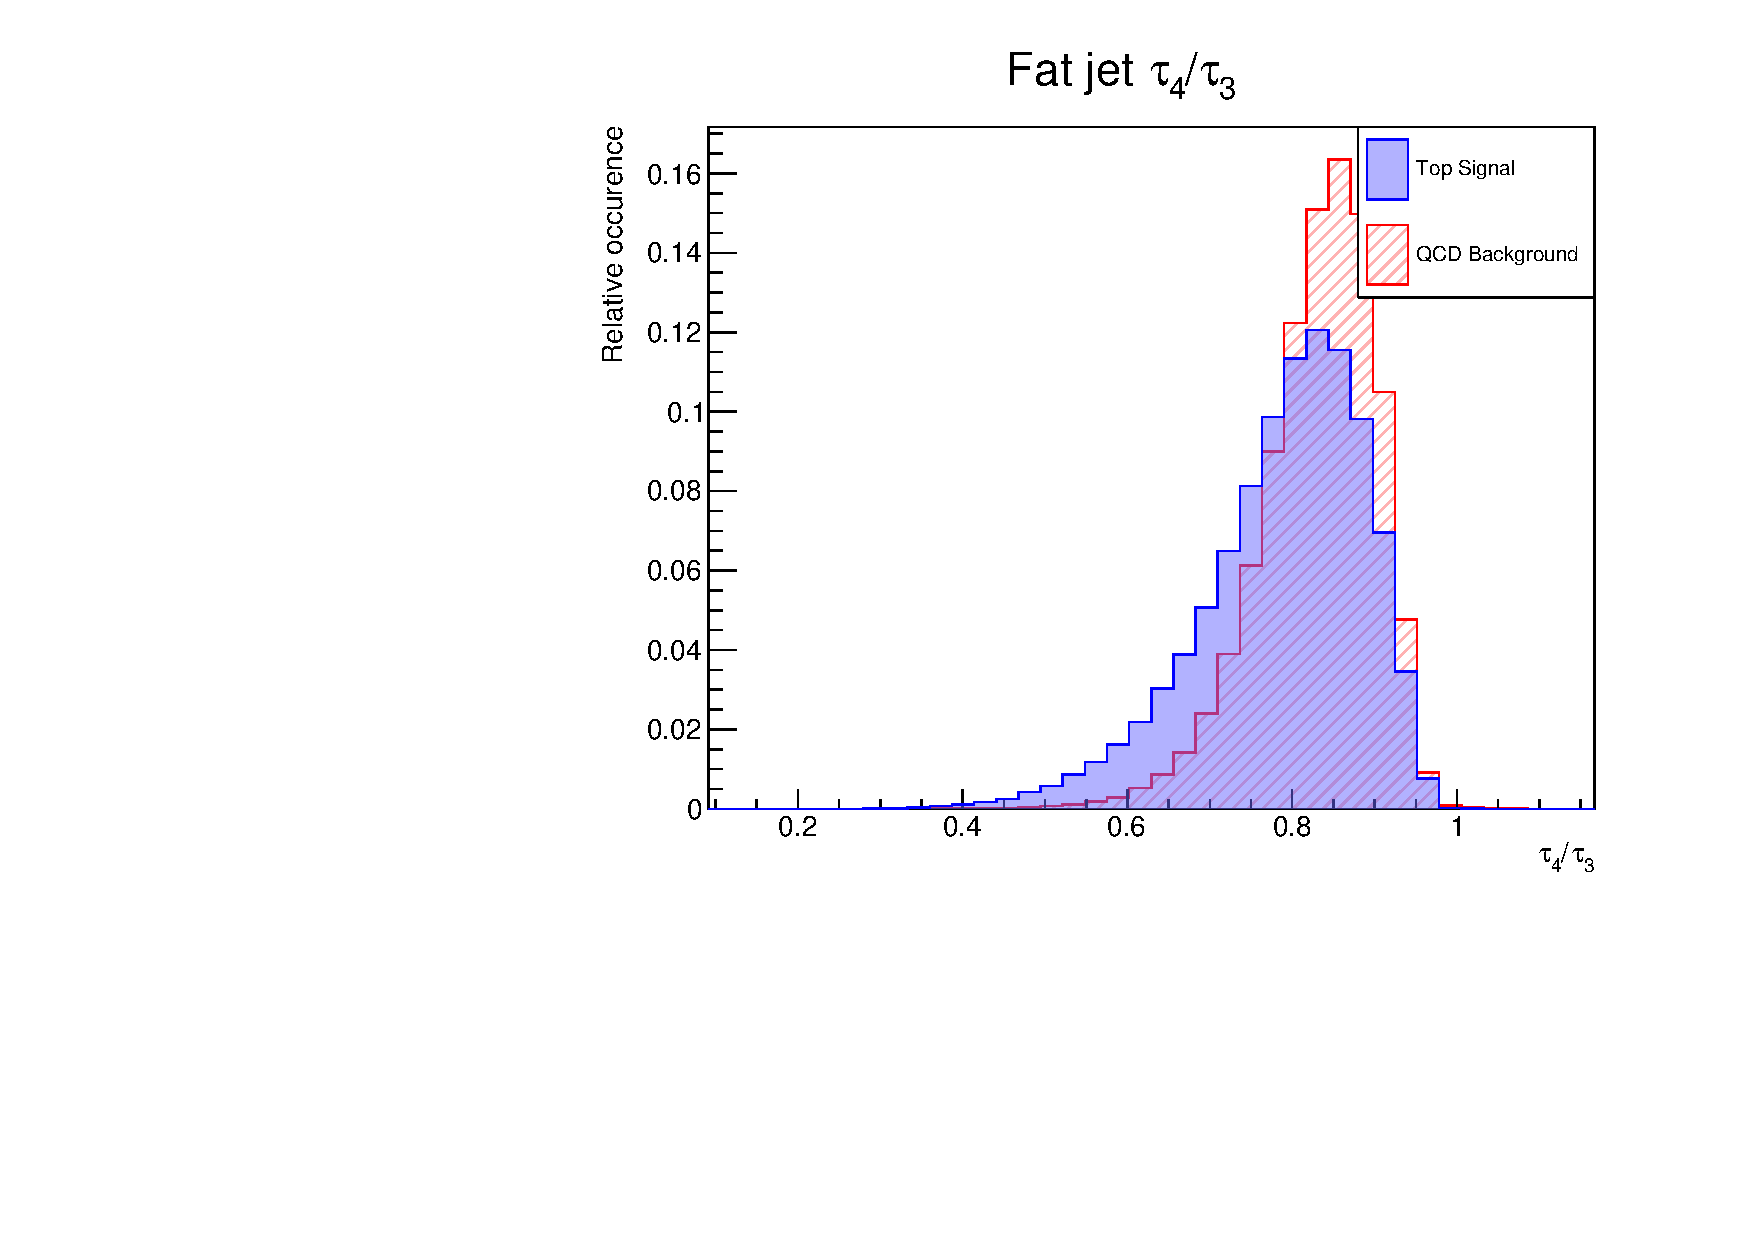
\includegraphics[width=0.8\textwidth]{../Figures/Results/top_distributions/top_tau43_distribution.pdf}
          \caption{}
         \label{fig:top_distribution_tau43}
     \end{subfigure}
     \begin{subfigure}[h]{0.49\textwidth}
         \centering
         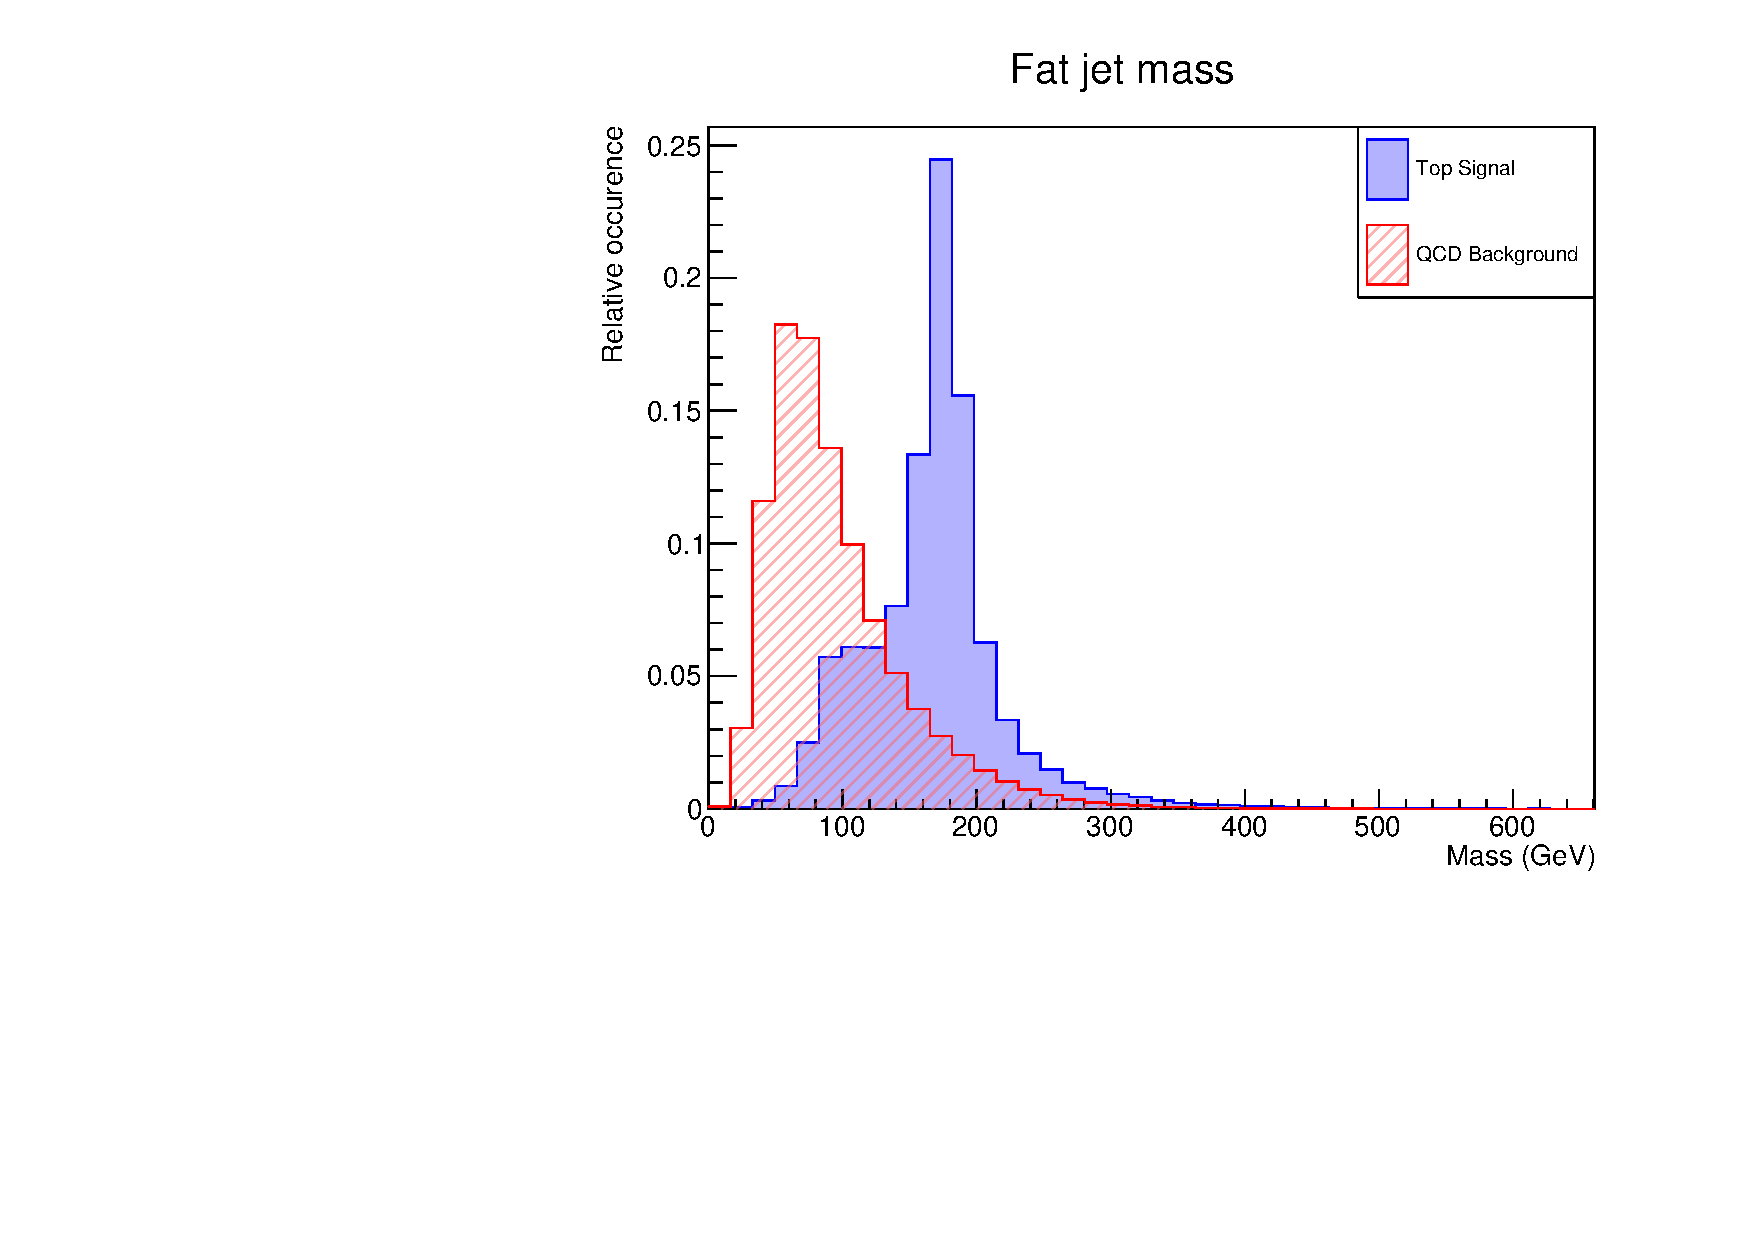
\includegraphics[width=0.8\textwidth]{../Figures/Results/top_distributions/top_mass_distribution.pdf}
          \caption{}
         \label{fig:top_distribution_mass}
     \end{subfigure}
     \caption{Distribution of (a)\;-\;(d) $\tau_N$, (e)\;-\;(g) $\tau_{N+1}/\tau_N$ ratios and (h) mass for the top and QCD fat jets in the training sample events.}
        \label{fig:top_distributions}
\end{figure}


% \hypsection{Discriminant variables}




















% \bibliographystyle{../../PhilReview} %%bib style found in bst folder, in bibtex folder, in texmf folder.
% \nobibliography{Zotero} %%bib database found in bib folder, in bibtex folder
% \nobibliography{../../Thesis_bib}
\biblio

\end{document}
